\newpage

\textbf{OLD VERSION BEFORE RESULTS - WE WILL DELETE SHORTLY}

\section{Market Formats} \label{market_formats}
mention other possibilities such as FBA and IEX, but here we'll just spell out CDA and Flow. \\

Our experiment investigates two market formats for trading assets. 

\subsection{Environment}
\textcolor{red}{We need an explanation of why the contract environment is more appropriate for our study than the usual stationary S/D partial eq environment.
I seem to recall that Brett's term paper on Flow Markets for the Market Design class explained why the usual environment wouldn't do, but I no longer remember. And our contract env with initiation and deadline times pretty much at the beginning and end of the period make it pretty similar to the usual environment.}

We propose the new contract environment for our laboratory experiments, where a single asset is traded on a single exchange. Traders receive a contract from the exchange near the beginning of each trading period. There are two types of such contracts: 1) buy contract, and 2) sell contract. For example, a buy contract might read ``Buy 300 shares at a price of 14 ECUs in 80 seconds". This means that 80 seconds from now, the exchange will buy up to 300 shares from your inventory at a price of 14 ECUs per share. Similarly, a sell contract that says ``Sell 400 shares at a price of 13 ECUs in 90 seconds" means that, in 90 seconds, the exchange will sell you up to 400 shares at the price of 14 ECUs per share. 

Contracts generate incentives to trade in this environment. For traders with a buy contract, it would be worthwhile to buy shares at a lower price than the contract price from other traders. Similarly, for traders with a sell contract, it would be profitable to sell shares at a higher price than the contract price.
Buyers will earn the difference between the contract price and the average buying price per share for their inventory while sellers will earn the difference between their average selling price and the contract price per share instead. When the contracts execute, traders' earnings will be reflected immediately in their cash account. 

The focus of the study is the behaviors of traders under different market formats, and the outcomes this behavior generates. Human participants play the role of traders and, at any instant, can choose to (a) send/cancel an order in the same direction of their contract,\footnote{ 
but not to exceed their contract quantity, in order to simplify the task and to avoid unintended loss due to over-trading.}
or (b) to send/cancel an order in the opposite direction of their contract after they accumulate some inventory in their contract direction. 

\subsection{Continuous Double Auction}
% Dan: show interface and walk thru order specs and processing

We now describe how continuous double auctions handle limit orders that are transmitted by trades. 

\subsubsection{Standard Limit Orders}

The standard limit orders are defined as messages with three parameters: a buy-sell indicator, a quantity $Q_{\max}$, and a limit price $P$. A standard buy limit order conveys the message ``Buy up to $Q_{\max}$ (shares) at a price of $P$ (dollars per share) or better." 

The continuous double auction (CDA), also known as the standard limit order book, works as follows. There is a \textit{limit order book} that sorts limit orders by price:  
bids are sorted from highest to lowest price and asks are sorted from lowest to highest price. 
Ties on price are resolved by time received: earlier orders take precedence over later orders at the same price. 
% The highest bid and the lowest ask are referred to as the \textit{best bid} and \textit{best ask}, respectively, and the difference between them is called the \textit{spread}.

Traders enter, replace, modify and cancel orders at any moment they choose and the CDA processes each limit order as it arrives. If the limit price locks (equals) or crosses (is beyond) the best contra-side price (e.g., if a new bid arrives with limit price equal to or higher than the current best ask) then the limit order immediately transacts at that best contra-side price, and the transacted quantity is removed from the order book. We say that limit order has been ``executed" or ``filled". On the other hand, if the price is no better than the current best same-side price, then the new order is added to the order book, behind other orders at the same price. 


\subsubsection{CDA User Interface}

Figure \ref{fig:cda_ui} shows one trader's CDA trading screen in our experiment. The top left sections shows an Active Contracts table, which describes the contract the trader got from the exchange around the beginning of this trading period. In the top middle section, the trader sets and submits orders. The horizontal axis denotes the quantity in shares and the vertical axis denotes prices in ECUs per share. The trader sets a \textit{buy} order by dragging the blue dot anywhere inside the grid to set the price and the quantity. Then the trader submits this buy order by clicking on the ``Send Buy" blue button. The blue-line segments describe her buy order graphically, as is shown in Figure \ref{fig:cda_ui}. Similarly, she sets a \textit{sell} order by dragging the red square anywhere inside the grid to set the price and the quantity and submits it by clicking on the ``Send Sell" red button. The active orders will show up in the Active Orders section in the second row of the leftmost column. She can submit a new order by first canceling her active orders in the same direction and then submit a new order at any time. 

\begin{figure}[!htbp]
    \centering
    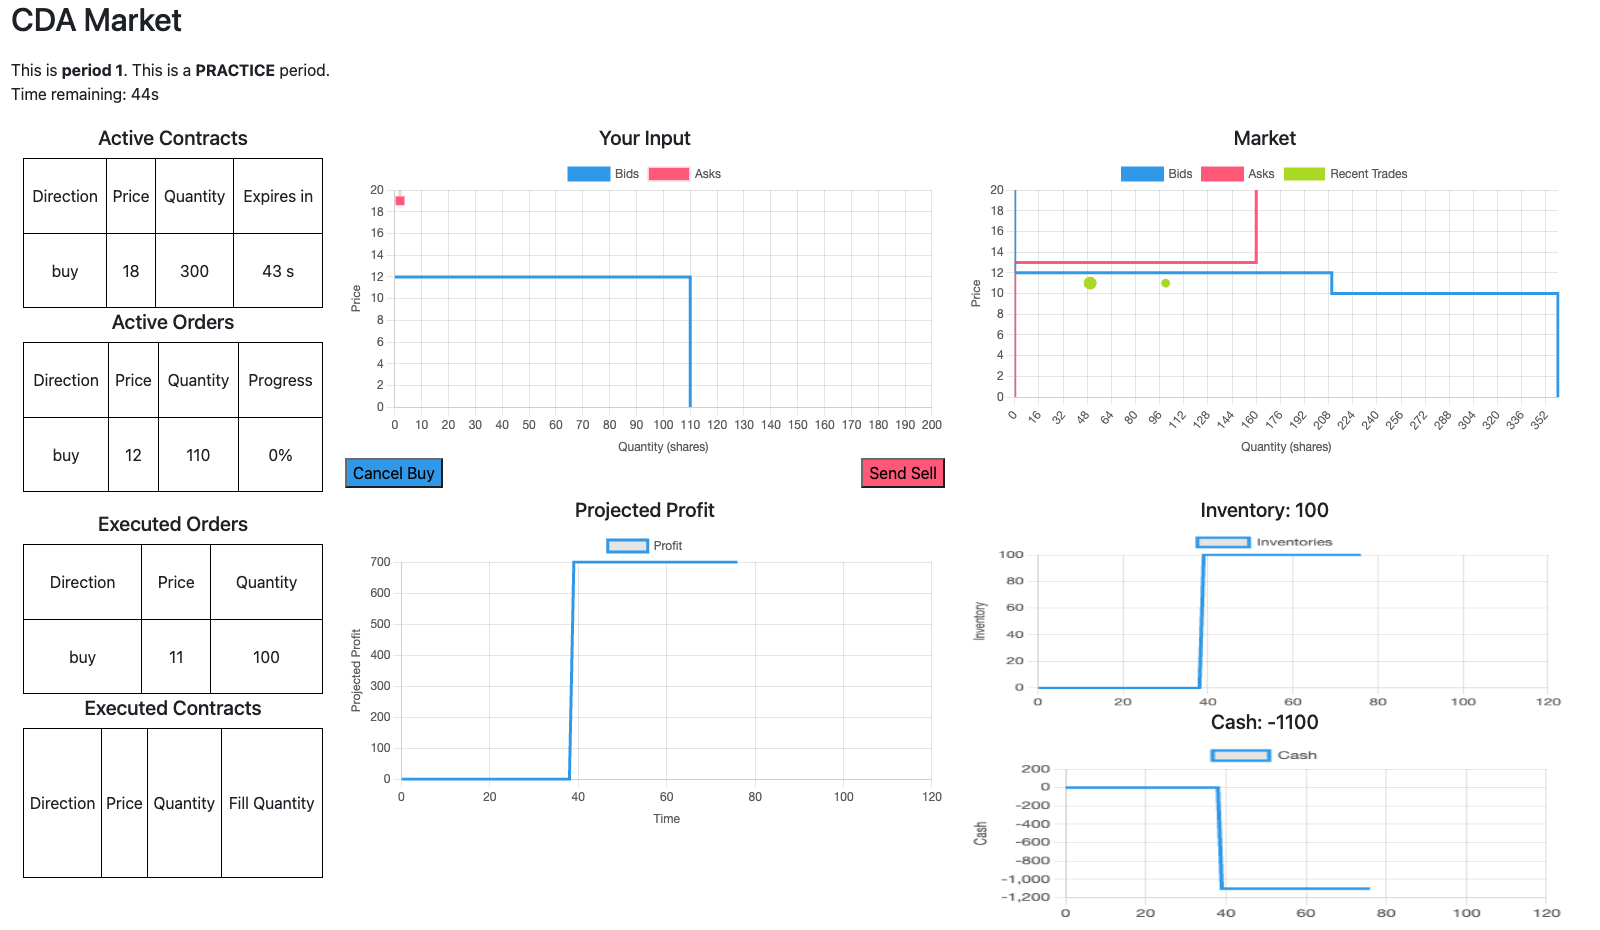
\includegraphics[width=\linewidth]{figures/cda_ui.png}
    \caption{CDA Trading Platform}
    \label{fig:cda_ui}
\end{figure}

In the top right Market section, the trader will see her own orders together with other traders'. The blue curve is the market demand and the red curve is the market supply. The intersection of them determines the market price as is shown on the vertical axis. Trades happen immediately when orders come into the market. The green dots indicate the most recent trades. The latest trade is represented by the largest dot. If the demand and supply do not cross each other inside the grid, there cannot be any trade at that point of trading period. If multiple buy orders tie in price, then the one that came in first will get executed first; same for sell orders. 

In the bottom right section, the trader will see how her inventory and cash change within each trading period. If any of her active orders gets fully executed, it will show up in the third row of the leftmost column in Figure \ref{fig:cda_ui}. In the bottom middle section, the trader will see her projected profit indicating what her profits would be if the active contract, if any, expires and the period ends right now; this provides a summary of her current state. Active contracts will move to the Executed Contracts section in the bottom left section. 

\subsection{Flow Trading}
% Dan: show interface and walk thru order specs and processing

Now we describe flowing trading format that is newly proposed by \cite{flow}.

\subsubsection{Continuous Scaled Limit Orders}
Let us first define the continuous scaled limit orders, CSLO, henceforth. The CSLO are messages with five parameters: a buy-sell indicator, a quantity $Q_{\max}$, two price levels $P_L$ and $P_H$ (with $P_L < P_H$), and the maximum trading speed $U_{\max}$. Such an order conveys the message, ``Buy up to a cumulative total of $Q_{\max}$ (shares) at maximum rate $U_{\max}$ (shares per hour) at prices between $P_L$ and $P_H$ (dollars per share)." The trading speed or flow demand $U(p(t))$ is a function of the market clearing price $p(t)$ given by 

$$U(p(t)) = \begin{cases}
	U_{max} & \text{if } p(t) < P_L \\
	\frac{P_H - p(t)}{P_H - P_L} U_{max} & \text{if } P_L \leq p(t) \leq P_H \\
	0 & \text{if } p(t) > P_H
\end{cases}$$

Similarly, the flow supply $U(p(t))$ is also a function of the market clearing price $p(t)$ given by 

$$U(p(t)) = \begin{cases}
	U_{max} & \text{if } p(t) > P_H\\
	\frac{p(t) - P_L}{P_H - P_L} U_{max} & \text{if } P_L \leq p(t) \leq P_H \\
	0 & \text{if } p(t) < P_L 
\end{cases}$$

If the price is strictly below (above) $P_L$ ($P_H$), the trader buys (sells) at the rate $U_{\max}$. If the price is strictly above (below) $P_H$ ($P_L$), the trader trades zero shares. If the price is between $P_L$ and $P_H$, the demand (supply) schedule is interpolated linearly, making its slope $\frac{(P_H - P_L)}{U_{\max}}$. 

% The cumulative quantity executed by time $t$ is 
% $$Q(t_0,t) = \int_{t_0}^{t_0+t} U(p(\tau)) d\tau$$

The market clears with continuous scaled limit orders by aggregating all the flow demands and flow supplies. The intersection of the downward sloping supply schedule and the upward sloping demand schedule, both of which are piece-wise linear functions of price, determines the unique clearing price and aggregate transaction rate. The individual transaction rate is determined by the intersection of the clearing price and individual flow supply/demand schedule. 

\subsubsection{FLOW User Interface}

Figure \ref{fig:flow_ui} shows one trader's FLOW trading screen. The top left section shows an Active Contracts table, which describes the contract the trader got from the exchange around the beginning of this trading period. In the top middle section, the trader sets and submits buy and sell orders. The horizontal axis denotes \textit{rate} in shares per second and the vertical axis denotes prices in ECUs per share. The trader sets a \textit{buy} order by moving the blue dot along the vertical axis to set the high price and dragging the blue square anywhere inside the grid to set the low price and the maximum rate. Then she enters the total number of shares she wants to buy in the box next to the ``Send Buy" blue button and submits it by clicking on that button. The blue-line segments describe her buy order graphically, as is shown in Figure \ref{fig:flow_ui}. Likewise, she sets a \textit{sell} order by moving the red dot along the vertical axis to set the low price and dragging the red square anywhere inside the grid to set the high price and the maximum rate. Then she enter the total number of shares she wants to sell in the box next to the ``Send Sell" red button and submits it by clicking on that button. The active orders will show up in the Active Orders section in the second row of the leftmost column. She can submit a new order by first canceling her active orders in the same direction and then submit a new order at any time. 

\begin{figure}[!htbp]
    \centering
    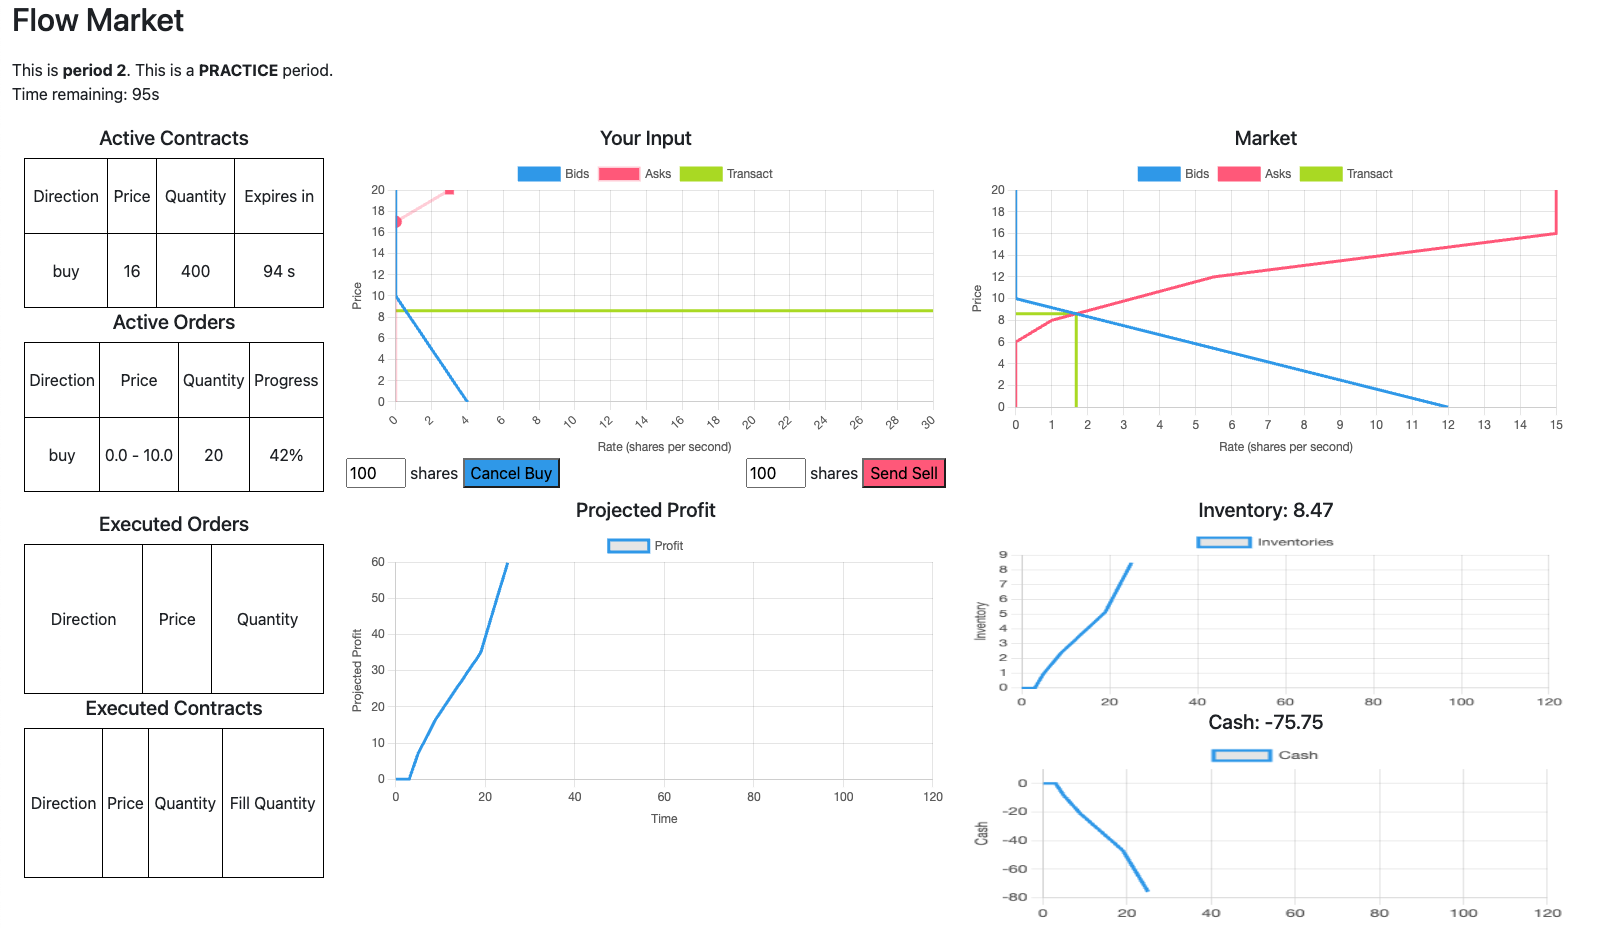
\includegraphics[width=\linewidth]{figures/flow_ui.png}
    \caption{FLOW Trading Platform}
    \label{fig:flow_ui}
\end{figure}

In the top right Market section, the trader will see her own orders together with other traders'. The blue curve is the market demand and the red curve is the market supply. The intersection of them determines the clearing price and the aggregate clearing rate. The green horizontal line in Market section extends into Your Input section and indicates the current transaction price. The x-coordinate of the intersection of this line and her individual order indicates her individual clearing rate. 

The bottom sections are the same as in the CDA trading platform. 

\subsection{Testable Hypotheses}
list the criteria we will use for market quality  --- 
allocative efficiency, price efficiency, price volatility, profit level and dispersion, ... ---
and for each criterion offer a hypothesis on which format will be better.




\section{Experiment Design} \label{experiment}


\subsection{Procedures}
The experiment was developed on oTree (\cite{otree}) and sessions were conducted at the LEEPS Laboratory of the University of California, Santa Cruz. Recruitment was implemented through LEEPS' ORSEE instance (\hyperlink{https://econlab.ucsc.edu/public/}{econlab.ucsc.edu}; \cite{subject}). Instructions were provided both on the computer screen and on paper.\footnote{Instructions were extensively discussed and piloted (with students and colleagues) to achieve a balance between clarity and reasonable length.} After 15 minutes of reading instructions, a video instruction was played with animations and annotations to clarify any confusions that subjects might have. Then two trial periods of 120 seconds each were launched during which subjects tested the interface with the understanding that their action had no consequences for their earning and would not comprise part of the formal experiment. Subjects were then given the option to publicly ask questions to the experimenters. The remainder of the session consisted of twenty trading periods of two minutes. In between trading periods, subjected received a summary screen displaying the profit history of each trading period. Each participant started with zero initial endowment at the beginning of each trading periods and final payments were based on the final wealth of all twenty trading periods, using an exchange rate of one thousand ECUs per dollar, plus a \$7 participant fee. The information was provided to subjects in the written instructions.

Although ending a trading period with negative profits was possible (i.e., having negative ECUs in the period), this happened only in 4.62\% of the cases (4.88\% in CDA and 4.37\% in FLOW) and subjects never left the laboratory with less than \$7. Members of a group (market) were not able to communicate with each other before, during, or after the experiment, nor did they learn the identity or characteristics of other participants. Payments were implemented following standard procedures of confidentiality. 

\begin{table}[htbp!]
    \centering
    \caption{Session Table}
    \begin{tabular}{cccc} \hline \hline
      Group & Format & \#Groups & \#Subjects \\ \hline
      1 & FLOW & 5 & 40 \\
      2 & CDA & 5 & 40 \\
      \hline \hline
    \end{tabular}
    \label{tab:design}
\end{table}


\subsection{Contract configurations}
% present the 5 configs that we use for both Flow and CDA sessions.
Figure \ref{fig:contract} illustrates the contract we used in our experiment. The blue curve represents the buy contracts and the red curve represents the sell contracts. An individual contract assigned to a trader is a line segment from either buy or sell contracts. We divide all twenty trading periods into five blocks, with four periods each. Within each block, traders always get the same contract. Between blocks, traders get different contacts. 


\begin{figure}[H]
    \centering
    \caption{Contract Design}
    \begin{subfigure}{.2\linewidth}
        \centering
        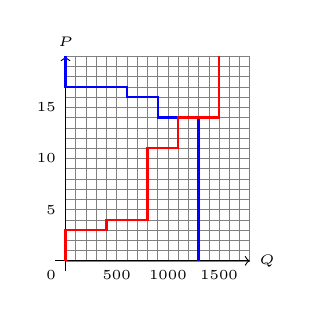
\begin{tikzpicture}[scale=.13]
            % create grid
            \draw[help lines] (0,0) grid (18,20);
            
            % Draw axes
            \draw[->] (-1,0) -- (18,0) node[font=\tiny,right] {$Q$};
            \draw[->] (0,-1) -- (0,20) node[font=\tiny,above] {$P$};
          
            % Draw step functions
            \draw[blue, thick] (0,20) -- (0,17) -- (6,17) -- (6,16) -- (9,16) -- (9,14) - - (13,14) -- (13,0) ;
            \draw[red, thick] (0,0) -- (0,3) -- (4,3) -- (4,4) -- (8,4) -- (8,11) --  (11,11) -- (11,14) -- (15,14) -- (15,20);
            
            % % Add labels
            \node[font=\tiny,below left] at (0,0) {$0$};
            \foreach \x in {5,10,15} {
              \node[font=\tiny,below] at (\x,0) {$\x00$};
            }
            \foreach \y in {5,10,15} {
              \node[font=\tiny,left] at (0,\y) {$\y$};
            }
        \end{tikzpicture}
        \subcaption{\tiny Block 1 \\ (T1 - T4)}
    \end{subfigure}%
    \begin{subfigure}{.2\linewidth}
        \centering
        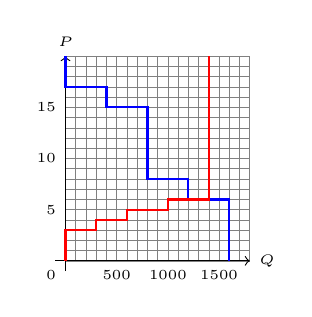
\begin{tikzpicture}[scale=.13]
            % create grid
            \draw[help lines] (0,0) grid (18,20);
            
            % Draw axes
            \draw[->] (-1,0) -- (18,0) node[font=\tiny,right] {$Q$};
            \draw[->] (0,-1) -- (0,20) node[font=\tiny,above] {$P$};
          
            % Draw step functions
            \draw[blue, thick] (0,20) -- (0,17) -- (4,17) -- (4,15) -- (8,15) -- (8,8) -- (12,8) -- (12,6) -- (16,6) -- (16,0);
            \draw[red, thick] (0,0) -- (0,3) -- (3,3) -- (3,4) -- (6,4) -- (6,5) -- (10,5) -- (10,6) -- (14,6) -- (14,20);
            
            % % Add labels
            \node[font=\tiny,below left] at (0,0) {$0$};
            \foreach \x in {5,10,15} {
              \node[font=\tiny,below] at (\x,0) {$\x00$};
            }
            \foreach \y in {5,10,15} {
              \node[font=\tiny,left] at (0,\y) {$\y$};
            }
        \end{tikzpicture}
        \subcaption{\tiny Block 2 \\ (T5 - T8)}
    \end{subfigure}%
    \begin{subfigure}{.2\linewidth}
        \centering
        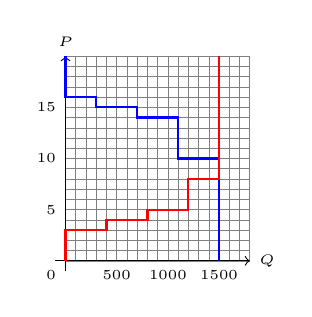
\begin{tikzpicture}[scale=.13]
            % create grid
            \draw[help lines] (0,0) grid (18,20);
            
            % Draw axes
            \draw[->] (-1,0) -- (18,0) node[font=\tiny,right] {$Q$};
            \draw[->] (0,-1) -- (0,20) node[font=\tiny,above] {$P$};
          
            % Draw step functions
            \draw[blue, thick] (0,20) -- (0,16) -- (3,16) -- (3,15) -- (7,15) -- (7,14) -- (11,14) -- (11,10) -- (15,10) -- (15,0);
            \draw[red, thick] (0,0) -- (0,3) -- (4,3) -- (4,4) -- (8,4) -- (8,5) -- (12,5) -- (12,8) -- (15,8) -- (15,20);
            
            % % Add labels
            \node[font=\tiny,below left] at (0,0) {$0$};
            \foreach \x in {5,10,15} {
              \node[font=\tiny,below] at (\x,0) {$\x00$};
            }
            \foreach \y in {5,10,15} {
              \node[font=\tiny,left] at (0,\y) {$\y$};
            }
        \end{tikzpicture}
        \subcaption{\tiny Block 3 \\ (T9 - T12)}
    \end{subfigure}%
    \begin{subfigure}{.2\linewidth}
        \centering
        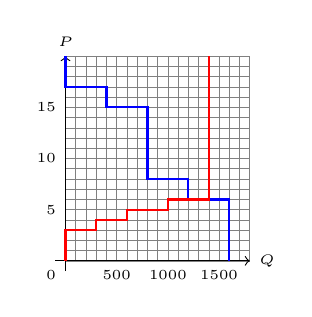
\begin{tikzpicture}[scale=.13]
            % create grid
            \draw[help lines] (0,0) grid (18,20);
            
            % Draw axes
            \draw[->] (-1,0) -- (18,0) node[font=\tiny,right] {$Q$};
            \draw[->] (0,-1) -- (0,20) node[font=\tiny,above] {$P$};
          
            % Draw step functions
            \draw[blue, thick] (0,20) -- (0,17) -- (4,17) -- (4,15) -- (8,15) -- (8,8) -- (12,8) -- (12,6) -- (16,6) -- (16,0);
            \draw[red, thick] (0,0) -- (0,3) -- (3,3) -- (3,4) -- (6,4) -- (6,5) -- (10,5) -- (10,6) -- (14,6) -- (14,20);
            
            % % Add labels
            \node[font=\tiny,below left] at (0,0) {$0$};
            \foreach \x in {5,10,15} {
              \node[font=\tiny,below] at (\x,0) {$\x00$};
            }
            \foreach \y in {5,10,15} {
              \node[font=\tiny,left] at (0,\y) {$\y$};
            }
        \end{tikzpicture}
        \subcaption{\tiny Block 4 \\ (T13 - T16)}
    \end{subfigure}%
    \begin{subfigure}{.2\linewidth}
        \centering
        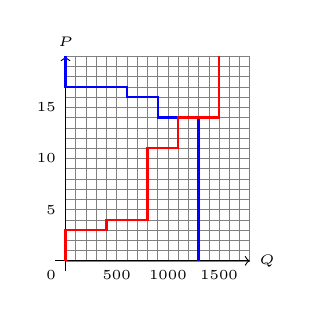
\begin{tikzpicture}[scale=.13]
            % create grid
            \draw[help lines] (0,0) grid (18,20);
            
            % Draw axes
            \draw[->] (-1,0) -- (18,0) node[font=\tiny,right] {$Q$};
            \draw[->] (0,-1) -- (0,20) node[font=\tiny,above] {$P$};
          
            % Draw step functions
            \draw[blue, thick] (0,20) -- (0,17) -- (6,17) -- (6,16) -- (9,16) -- (9,14) - - (13,14) -- (13,0) ;
            \draw[red, thick] (0,0) -- (0,3) -- (4,3) -- (4,4) -- (8,4) -- (8,11) --  (11,11) -- (11,14) -- (15,14) -- (15,20);
            
            % % Add labels
            \node[font=\tiny,below left] at (0,0) {$0$};
            \foreach \x in {5,10,15} {
              \node[font=\tiny,below] at (\x,0) {$\x00$};
            }
            \foreach \y in {5,10,15} {
              \node[font=\tiny,left] at (0,\y) {$\y$};
            }
        \end{tikzpicture}
        \subcaption{\tiny Block 5 \\ (T17 - T20)}
    \end{subfigure}
    \label{fig:contract}
\end{figure}

